
\section{Analytic Solution: Log Utility Case}
\label{sec:log_utility.sec}

In this section, we consider the case of log utility, $\psi=\gamma=1$.
This special case allows us to characterize in closed form how beliefs affect asset
prices and labor demand in equilibrium. We use this analytic solution to highlight the
mechanisms through which belief heterogeneity amplifies business-cycle fluctuations and how it affects trading patterns.
We return to more general preferences in the quantitative analysis.

\subsection{Beliefs, asset prices, and labor demand}\label{sec:beliefs_asset_prices_labor_demand.sec}
\q{AssetPrices}{
\paragraph{Asset prices.}

Under log utility, both the consumption--wealth ratio and the price--dividend ratio are
constant:
\begin{equation}
c_i(X,s)=1-\beta,
\qquad
q(X,s)=\frac{\beta}{1-\beta},
\end{equation}
which follows directly from
Equations~\eqref{eq: consumption_wealth_ratio} and
\eqref{eq: mkt_clearing_markov}.
As a result, the return on the risky asset is proportional to dividend growth:
\[
R_{r,t+1}
=
\frac{1+q_{t+1}}{q_t}\frac{\pi_{t+1}}{\pi_t}
=
\beta^{-1}\frac{\pi_{t+1}}{\pi_t}.
\]

Using the expression for dividend growth derived in
Equation~\eqref{eq: dividend_growth}, the gross return on the risky asset can be written as
\begin{equation}
R_r(X,s,s')
=
\beta^{-1}
\,
x_s
\frac{x_{s'}-\alpha\mathcal L'(X,s)}{x_s-\alpha\mathcal L}
\left(
\frac{\mathcal L'(X,s)}{\mathcal L}
\right)^{\frac{\alpha}{1-\alpha}}.\nonumber
\end{equation}

The risk-free rate equals the risk-neutral expectation of the return on the risky asset.
Using the fact that $\mathcal L'(X,s)$ is the risk-neutral expectation of $x_{s'}$, we
obtain
\begin{equation}
R_f(X,s)
=
\beta^{-1}
\,
x_s
\frac{(1-\alpha)\mathcal L'(X,s)}{x_s-\alpha\mathcal L}
\left(
\frac{\mathcal L'(X,s)}{\mathcal L}
\right)^{\frac{\alpha}{1-\alpha}}.\nonumber
\end{equation}}

The next proposition summarizes the relationship between the risk-free rate, the risk
premium, and the risk-neutral expectation of productivity growth.

\q{Prop_Asset_Prices}{\begin{proposition}[Risk-free rate and risk premium]
\label{prop:asset_prices}
Given $\mathcal L'(X,s)$:
\begin{enumerate}[(i)]
\item
The risk-free rate satisfies
\begin{equation}
R_f(X,s)
=
(1-\alpha)\frac{x_s}{\beta}
\frac{\mathcal L'(X,s)^{\frac{1}{1-\alpha}}}
{x_s\mathcal L^{\frac{\alpha}{1-\alpha}}
-
\alpha\mathcal L^{\frac{1}{1-\alpha}}}.
\end{equation}

\item
The conditional risk premium is
\begin{equation}
\mathbb E_s\!\left[R_r^e(X,s,s')\right]
=
\frac{1}{1-\alpha}
\frac{\mathbb E_s[x_{s'}]-\mathcal L'(X,s)}{\mathcal L'(X,s)},
\label{eq:risk_premium}
\end{equation}
which is decreasing in $\mathcal L'(X,s)$.
\end{enumerate}
\end{proposition}}

\q{Implications_Asset_Prices}{Proposition~\ref{prop:asset_prices} shows that asset prices are fully pinned down by the
current state $(X,s)$ and the risk-neutral expectation of productivity growth,
$\mathcal L'(X,s)$. Intuitively, a higher $\mathcal L'(X,s)$ reflects either
higher expected productivity growth or lower aggregate risk, both of which raise the
risk-free rate.

At the same time, interest rates are decreasing in current productivity growth $x_s$.
As discussed in Section~\ref{sec:analysis.sec4}, the timing of hiring induces mean
reversion in dividends: following a negative productivity shock, expected dividend
growth is high, raising equilibrium interest rates.

Finally, the risk premium is increasing in the wedge between physical and risk-neutral
expectations of productivity growth. Conditional on $\mathbb E_s[x_{s'}]$, a lower
$\mathcal L'(X,s)$ corresponds to a larger risk adjustment and therefore a higher
expected excess return.}


\paragraph{A demand--supply representation.}
Proposition~\ref{prop: risk} implies that firm's labor demand, as summarized by risk-neutral expected growth, and asset prices are tightly connected. 
Next, we solve for the equilibrium $\mathcal{L}'(X,s)$ by translating the market clearing conditions into a demand and supply system.%, where the quantity variable is aggregate volatility risk, and the price variable is $\mathcal{L}'(X,s)$. 

This demand and supply of risk representation is a convenient transformation of the asset-market clearing condition \eqref{eq: mkt_clearing_markov}: multiply both sides of the condition for risky assets by $\sigma_s[R_r(X,s,s')]$, and use that $\sigma_s[R_{i}(X,s,s')] = \omega_{i}(X,s) \sigma_s[R_{r}(X,s,s')]$, to obtain:
    

% Unlike when hiring occurs after productivity is realized, here, labor demand and asset prices are determined jointly. 
% Proposition \ref{prop: asset_prices} shows that the risk-free rate and the risk premium can be deduced from the current productivity growth, $x_s$, and the lagged and current period's LDF, $\mathcal{L}$ and $\mathcal{L}'(X,s)$. 
% The risk free rate, $R_{b}(X,s)$, is increasing in $\mathcal{L}'(X,s)$ and decreasing in $x_s$ whereas the risk premium $\mathbb{E}_s[R_{r}^e(X,s,s')]$ moves in the opposite direction of $\mathcal{L}'(X,s)$. 
% The formula reveals that ceteris paribus, periods of low-risk premia are associated with high labor demand. 
% Of course, the LDF is endogenous; it is a function of market beliefs. 


% Next, we solve for the equilibrium LDF by translating the market clearing conditions into a demand and supply system, where the quantity variable is the risk in the economy's aggregate surplus claim, and the price variable is the LDF. The equilibrium of this demand and supply system yields the equilibrium LDF and, thus, pins down all asset prices and labor demand. This demand and supply of risk representation is a convenient transformation of the asset-market clearing conditions \eqref{eq: mkt_clearing_markov}: multiply both sides of the condition for risky assets by $\sigma_s[R_r(X,s,s')]$, and use that $\sigma_s[R_{i,n}(X,s,s')] = \omega_{i}(X,s) \sigma_s[R_{r}(X,s,s')]$, to obtain:
\begin{equation*}
    \underbrace{\sum_{i=1}^I \eta_i \sigma_s[R_{i}(X,s,s')]}_{\text{demand for risk}} =  \underbrace{\sigma_s[R_r(X,s,s')]}_{\text{supply of risk}}.
\end{equation*}
The left of the expression is the \textit{demand for risk}, corresponding to the volatility of households' wealth. 
The right-hand side represents the \textit{supply of risk}, that is, the volatility of assets in positive net supply.
The following proposition expresses the demand and supply of risk as a function of $\mathcal{L}'(X,s)$.
\begin{proposition}[The demand and supply of risk] \label{prop: risk} Suppose $x_L > \alpha x_H $. Then,
\begin{enumerate}[(i)]
    \item The supply of risk is
    \begin{equation}
        \sigma_s[R_r(X,s,s')] = \frac{\sigma_s[x_{s'}] }{\beta} \frac{x_s}{x_{s} - \alpha \mathcal{L} } \frac{\mathcal{L}'(X,s)^\frac{\alpha}{1-\alpha}}{\mathcal{L}^\frac{\alpha}{1-\alpha} }.
    \end{equation}
    \item The demand for risk is
    \begin{equation}
        \sum_{i=1}^I \eta_i \sigma_s[R_{i}(X,s,s')] =  \sigma_s[x_{s'}] R_f(X,s) \left[\frac{\overline{p}^m_{sH}(X,s)}{\mathcal{L}'(X,s) - x_L}  -\frac{\overline{p}^m_{sL}(X,s)}{x_H-\mathcal{L}'(X,s)} \right],
    \end{equation}
    where $\overline{p}_{ss'}^{m}(X,s) \equiv \sum_{i=1}^I \eta_i p_{ss'}^i$.
\end{enumerate}

\end{proposition}
Proposition \ref{prop: risk} implies that the supply of risk increases while the demand for risk decreases with the $\mathcal{L}'(X,s)$, as shown in Figure \ref{fig: risk_eq}. 
\begin{figure}[t!]
    \begin{minipage}[t!]{\textwidth}
      \begin{minipage}[b]{0.5\textwidth}
        \centering 
        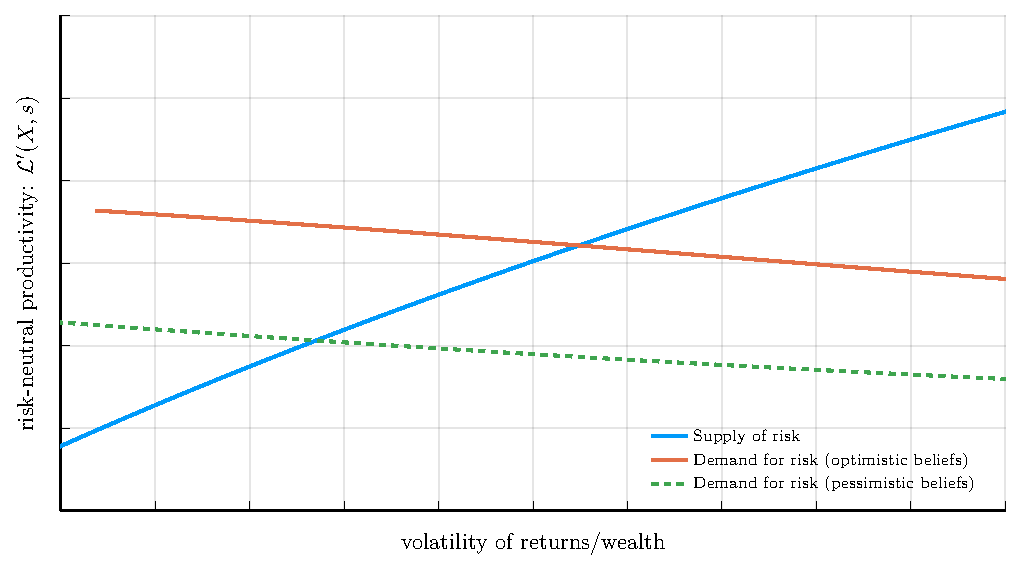
\includegraphics[width=0.99\textwidth]{figures/risk_equilibrium_inv.pdf}
            \caption{Market for risky assets}\label{fig: risk_eq}
        \end{minipage}
        \hfill
      \begin{minipage}[b]{0.5\textwidth}
        \centering
        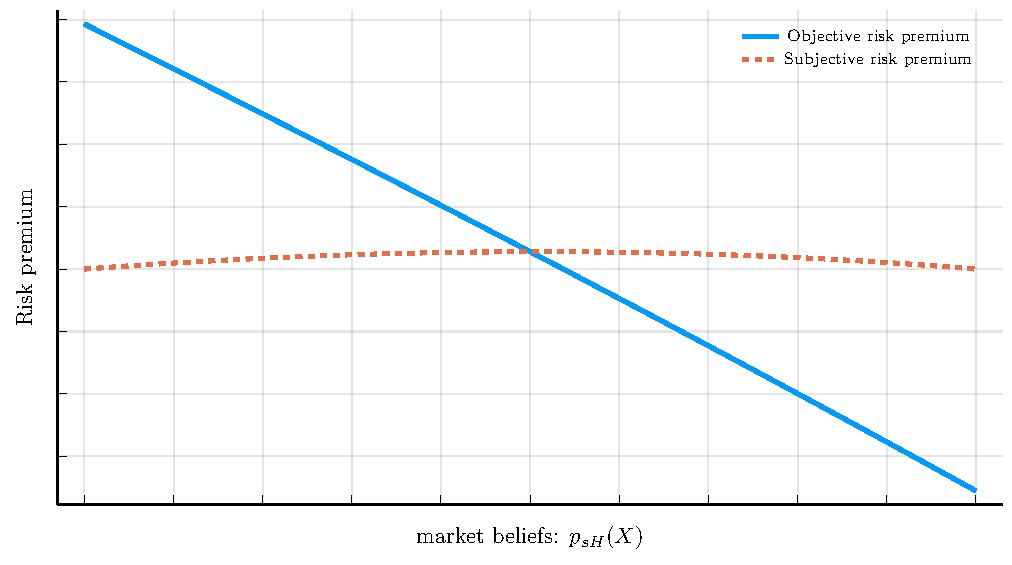
\includegraphics[width=0.99\textwidth]{figures/obj_subj_risk_premia.pdf}
            \caption{Beliefs and risk premia}\label{fig: obj_subj_risk_premia}
      \end{minipage}
      
      \end{minipage}    

    \end{figure}
Recall return volatility is proportional to dividend volatility. 
The supply of risk increases with $\mathcal{L}'(X,s)$ because dividend volatility increases with $\mathcal{L}'(X,s)$ due to the operating leverage channel. 
As firms hire more labor, profits are more exposed to productivity shocks, leading to higher volatility. 

The demand for risk is decreasing in $\mathcal{L}'(X,s)$. As shown in Proposition \ref{prop:asset_prices}, the risk premium is inversely related to $\mathcal{L}'(X,S)$, so investors are more willing to hold risky assets when the risk premium is high. 
The demand for risk is also a function of \textit{market beliefs}, a weighted average of investors' beliefs, $\overline{p}_{ss'}^m(X,s)$.
As market beliefs become more optimistic, investors are willing to hold more risky assets for a given risk premium.

Figure \ref{fig: risk_eq} illustrates how we can exploit this demand system representation to explain the effects of changes in market beliefs: 
When market beliefs become more pessimistic, there is a decline in the demand for risk, which leads to a decrease in the risk-neutral expected growth and, ultimately, a drop in employment. 

The following corollary formally demonstrates this by presenting the solution to the equilibrium risk-neutral expected growth as a function of market beliefs.
\begin{corollary}[Labor demand factor]\label{cor: Eprime} The risk-neutral expectation of productivity growth $\mathcal{L}'(X,s)$ is given by: 
\begin{equation}
    \mathcal{L}'(X,s)=\Gamma(X,s) - \sqrt{\Gamma(X,s)^{2}-\frac{1}{\alpha}  x_L x_H}.\nonumber
\end{equation}
where $\Gamma(X,s)$ is a function of market beliefs:
\[  
\Gamma(X,s)\equiv  \frac{\overline{p}^m_{sH}(X,s)}{2} \left(\frac{x_L}{\alpha} + x_H \right)+ \frac{\overline{p}^m_{sL}(X,s)}{2}\left(  x_L + \frac{x_H}{\alpha} \right).
\]
\end{corollary}
The key implication of Corollary~\ref{cor: Eprime} is that the risk-neutral expectation of productivity growth is \emph{entirely} determined by market beliefs. 
As a result, fluctuations in market beliefs translate directly into fluctuations in labor demand through firms' hiring decisions. 
Moreover, because market beliefs are a wealth-weighted average of individual beliefs, they depend on the distribution of wealth across investors. 
Changes in the wealth distribution therefore affect production through their impact on aggregate beliefs, providing a direct link between asset prices, labor demand, and the evolution of wealth inequality.


\q{RealEffects}{
\paragraph{The real effects of market beliefs.}

We have seen that, in our baseline economy, asset prices and labor demand are jointly
determined. The timing of hiring decisions is crucial for this result. To make this
point explicit, the next proposition shows that market beliefs have no real effects
when firms are allowed to adjust labor after productivity is realized.

\begin{proposition}[Real effects of market beliefs]
\label{prop:real_effects_beliefs}
Suppose firms choose hours after observing current productivity. Then hours, detrended
profits, and the return on the risky asset are independent of market beliefs:
\small
\begin{equation}
h(X,s)
=
\left(\frac{\alpha x_s}{\xi}\right)^{\frac{1}{1-\alpha}},
\qquad
\pi(X,s)
=
(1-\alpha)
\left(\frac{\alpha}{\xi}\right)^{\frac{\alpha}{1-\alpha}}
x_s^{\frac{1}{1-\alpha}},
\qquad
R_r(X,s,s')
=
\frac{x_s}{\beta}
\left(\frac{x_{s'}}{x_s}\right)^{\frac{1}{1-\alpha}}.
\end{equation}
\normalsize
Fluctuations in market beliefs affect the risk-free rate and the risk premium, but they
do not affect real variables or the expected return and volatility of the risky asset
under the objective measure.
\end{proposition}

Proposition~\ref{prop:real_effects_beliefs} establishes a form of
\emph{macro--finance separation} \citep{T00}: in the absence of a hiring friction,
belief-driven fluctuations in risk premia have asset-pricing implications but no real
effects on employment or output.

The timing assumption on hiring breaks this separation. When labor must be chosen in
advance, hiring is risky from the firm's perspective. An increase in optimism compresses
the risk premium, raises the value of risky assets, and---through the firm's optimality
condition---leads to higher employment. In this case, asset prices and labor demand are
simultaneously determined.

Absent fluctuations in market beliefs, employment would be constant in this economy,
consistent with the labor volatility puzzle documented by
\citet{shimer2010labor}. Section~\ref{sec:quantitative} explores the quantitative
implications of this mechanism by assessing how much labor volatility the model can
generate under empirically realistic fluctuations in beliefs.
}

\q{BeliefsAndRiskPremia}{
\paragraph{Beliefs and risk premia.}

Fluctuations in market beliefs generate movements in both risk premia
and labor demand. Why does optimism lead to changes in risk premia?

To answer this question, it is useful to distinguish between \emph{subjective} and
\emph{objective} risk premia. 
With a representative investor, the subjective risk premium is simply given by:
\begin{equation}
\mathbb E_{i,s}\!\left[R_r^e(X,s,s')\right]
\approx
\operatorname{Var}_{i,s}\!\left[R_r^e(X,s,s')\right].
\end{equation}
Thus, absent changes in perceived volatility, shifts in beliefs about average
productivity growth have little effect on the subjective risk premium in this case.

In contrast, the objective risk premium responds to differences in first moments. Using
the equilibrium expressions derived above, it can be written as
\begin{equation}
\mathbb E_s\!\left[R_r^e(X,s,s')\right]
=
\mathbb E_{i,s}\!\left[R_r^e(X,s,s')\right]
-
\frac{\mathbb E_{i,s}[x_{s'}]-\mathbb E_s[x_{s'}]}
{(1-\alpha)\mathcal L'(X,s)}.
\end{equation}
When investors become optimistic, they expect higher future dividends and bid up asset
prices. From the perspective of a rational investor, higher prices imply lower expected
returns going forward, compressing the objective risk premium.

Figure~\ref{fig: obj_subj_risk_premia} illustrates this mechanism. An increase in optimism,
captured by a rise in market beliefs $\overline p_{sH}^m(X,s)$, substantially reduces the
objective risk premium, while having a more muted effect on the subjective risk
premium. This pattern is consistent with empirical evidence documenting large movements
in expected returns with relatively stable subjective risk perceptions (see, e.g.,
\citealt{de_la_o_subjective_2021} and \citealt{nagel2023dynamics}).
}

\paragraph{The evolution of market beliefs.}
We have seen how market beliefs are determined by the wealth distribution. Next, we show how the wealth distribution evolves over time:
\begin{proposition}[Wealth dynamics]\label{prop: dynamics_beliefs} 
    The wealth share of investor $i\in \mathcal{I}$ evolves as:
        \begin{equation}
        \eta_i'(X,s,s') = \eta_i \frac{p^i_{ss'}}{\overline{p}^m_{ss'}(X,s)}.
    \end{equation}
    % \begin{enumerate}[(i)]
%     \item the wealth share of investor $i\in \mathcal{I}$ evolves as:
%     \begin{equation}
%     \eta_i'(X,s,s') = \eta_i \frac{p^i_{ss'}}{\overline{p}^m_{ss'}(X,s)},
% \end{equation}

%     \item market beliefs are:
%     \begin{equation}
%         \overline{p}^m_{s'H}(X',s') = \sum_{i=1}^I \eta_i \frac{p^i_{ss'}}{\overline{p}^m_{ss'}(X,s)} p_{s'H}^i.
%     \end{equation}
% \end{enumerate}
\end{proposition}
Proposition \ref{prop: dynamics_beliefs} shows that the wealth of household $i$ increases when she assigns a greater likelihood to the realized state than market beliefs. 

Next, we present a taxonomy of belief types. 
In particular, we discuss how different belief structures classified according to our taxonomy impact business cycles.

\subsection{Belief taxonomy and business-cycle properties}
\label{sec:belief_taxonomy.sec}

Although a large literature documents departures from full-information rational
expectations \citep{greenwood_expectations_2014, coibion2015information}, there is no
consensus on how precisely belief dynamics deviate from rational expectations.\footnote{Some
studies emphasize over-extrapolation \citep{bordalo2020overreaction, fuster2010natural},
as in models with diagnostic expectations \citep{bordalo2018diagnostic} or fading memory
\citep{nagel2022asset}. Others emphasize under-reaction, such as sticky information
\citep{mankiw2010imperfect}, cognitive discounting \citep{gabaix2019behavioral}, and
level-$k$ thinking \citep{farhi2019monetary}.} This section classifies belief structures
and shows how each maps into distinct business-cycle implications. We organize the
analysis around the following taxonomy.

\begin{definition}[Taxonomy of beliefs]
\label{def: belief_taxonomy}
\q{Taxonomy}{
Household $i$ is \emph{optimistic} (\emph{pessimistic}) relative to a benchmark belief
$o$ in state $s$ if $p_{sH}^i > p_{sH}^o$ ($p_{sH}^i < p_{sH}^o$). We further distinguish
two classes of belief dynamics:
\begin{enumerate}[(i)]
\item \textbf{Rank-preserving beliefs}: household $i$ is optimistic or pessimistic
relative to $o$ in all states.
\item \textbf{Rank-alternating beliefs}: household $i$ is optimistic relative to $o$ in
one state but pessimistic in the other.
\end{enumerate}
}
\end{definition}

The benchmark belief $o$ can represent either rational expectations or the beliefs of
another household. This taxonomy allows us to characterize how different belief
structures affect both the amplitude and the phase of business-cycle fluctuations.

\paragraph{Homogeneous beliefs.}

With homogeneous beliefs, the risk-neutral expectation of productivity growth,
$\mathcal L'(X,s)$, depends only on current productivity. 
Therefore, the models lacks an internal propagation mechanism, as there is no variation in hours in the absence of changes in productivity growth. 
Moreover, if
investors believe productivity growth is i.i.d., so that $p_{LH}^i=p_{HH}^i$, then
$\mathcal L'(X,s)$ and, consequently, hours are constant over time.

Away from i.i.d.\ beliefs, homogeneous beliefs can either amplify or dampen fluctuations. Figure~\ref{fig: hom_beliefs} illustrates
this point by simulating four periods of recession within a twenty-period interval for
five belief specifications: rational expectations
($p_{ss'}^i=p_{ss'}$ for all $s,s'$); two rank-preserving cases---always optimistic
($p_{sH}^i>p_{sH}$ for all $s$) and always pessimistic ($p_{sH}^i<p_{sH}$ for all $s$);
and two rank-alternating cases---\emph{extrapolative} beliefs, defined as optimistic in
booms and pessimistic in recessions, and \emph{contrarian} beliefs, defined as
pessimistic in booms and optimistic in recessions.

Optimistic rank-preserving beliefs amplify expansions but dampen recessions relative to
rational expectations, while pessimistic rank-preserving beliefs have the opposite
effect. Thus, rank-preserving beliefs generate state-dependent amplification.

Rank-alternating beliefs operate differently. Under extrapolative beliefs, optimism in
booms and pessimism in recessions magnify the amplitude of the cycle. By contrast, contrarian beliefs dampen fluctuations by reducing
labor demand in booms and supporting it in recessions. Overall, extrapolative beliefs are
the belief structure that most strongly amplifies business-cycle fluctuations relative
to rational expectations.

\begin{figure}[t!]
    \centering
            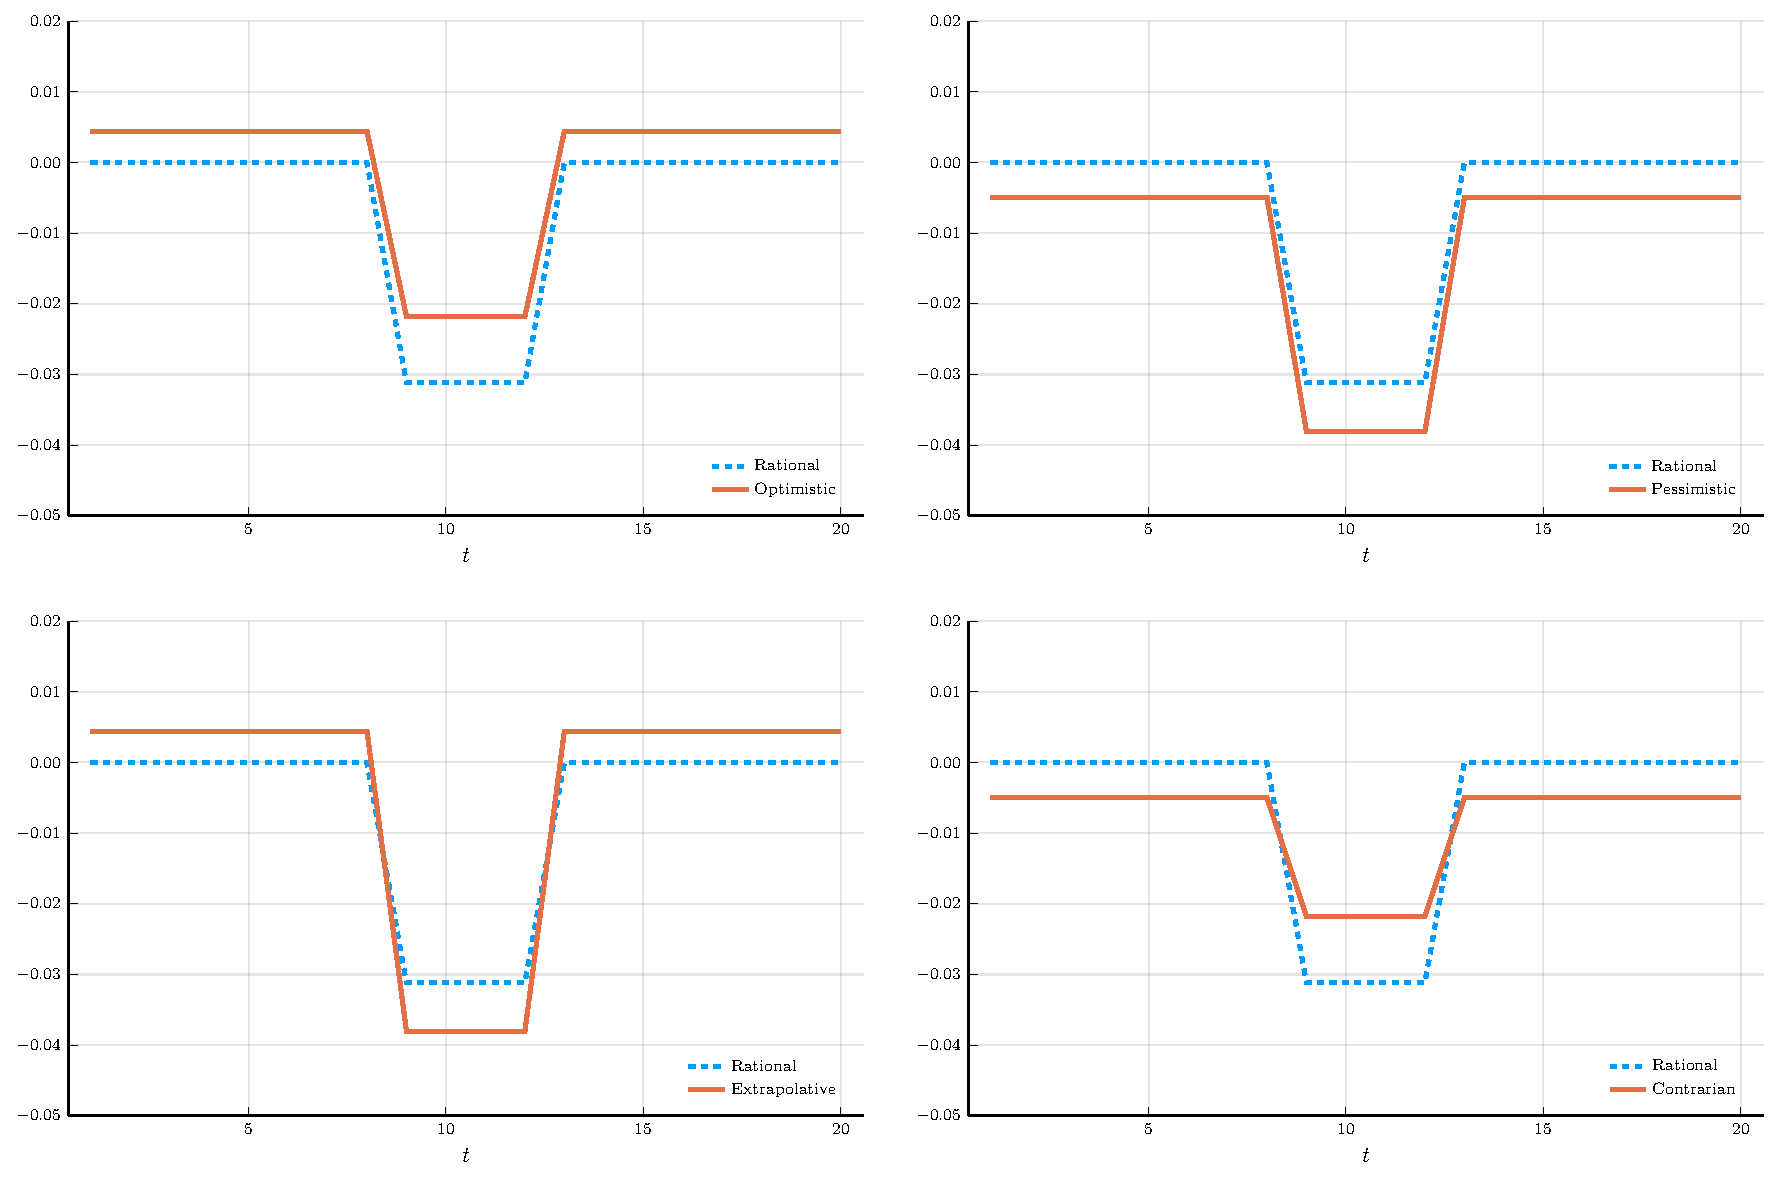
\includegraphics[width=0.90
            \textwidth]{figures/simul_hom_beliefs.pdf}
    \caption{Homogeneous beliefs}
    \caption*{  \scriptsize 
    Note: examples of cycles (four periods of bad shocks with sixteen periods of expansions) for log labor hours with homogeneous beliefs: rational, always optimistic (top-left panel), always pessimistic (top-right panel), extrapolative (bottom-left panel), and contrarian (bottom-right panel) beliefs. \par} 
    \vspace{0.0cm}
    \label{fig: hom_beliefs}
\end{figure}

\paragraph{Heterogeneous beliefs.}

Next, we investigate the role of belief heterogeneity. 
It is well known that RBC models typically have very weak internal propagation mechanisms \citep{cogley1995output}.
With heterogeneous beliefs and labor chosen one period in advance, the model features an important internal propagation mechanism: the wealth distribution, and market beliefs, evolve over time even without changes in the productivity state.
% The model now features an internal propagation mechanism, as the wealth distribution, and market beliefs, evolve over time even without changes in the productivity state.
From Proposition~\ref{prop: dynamics_beliefs}, optimists accumulate wealth during booms and lose
wealth during downturns. This observation is key to understanding the model dynamics.

\begin{corollary}\label{cor:het_dynamics}
If beliefs are heterogeneous, then:
\begin{itemize}
\item Conditional on remaining in the same state, the risk-neutral expectation of
productivity growth $\mathcal L$ increases (decreases) over time in the high-growth
(low-growth) state.
\item Consider an initial state $(X,H)$ and a transition from $H$ to $L$ at some future
date. Then:
\begin{itemize}
\item If beliefs are \emph{rank-preserving}, a longer boom leads to a smaller subsequent
decline in output.
\item If beliefs are \emph{rank-alternating}, a longer boom leads to a larger subsequent
decline in output.
\end{itemize}
\end{itemize}
\end{corollary}

% \begin{proof}
% See Appendix~\ref{app: proof_cor_het_dynamics}.
% \end{proof}

With belief heterogeneity, the economy evolves even in the absence of changes in
productivity growth. 
During booms, optimistic investors accumulate wealth, causing market beliefs to become
more optimistic relative to rational expectations and increasing labor demand. The
opposite occurs during prolonged low-growth phases, when pessimistic investors gain
wealth and market beliefs tilt toward pessimism.

\begin{figure}[t!]
    \centering
            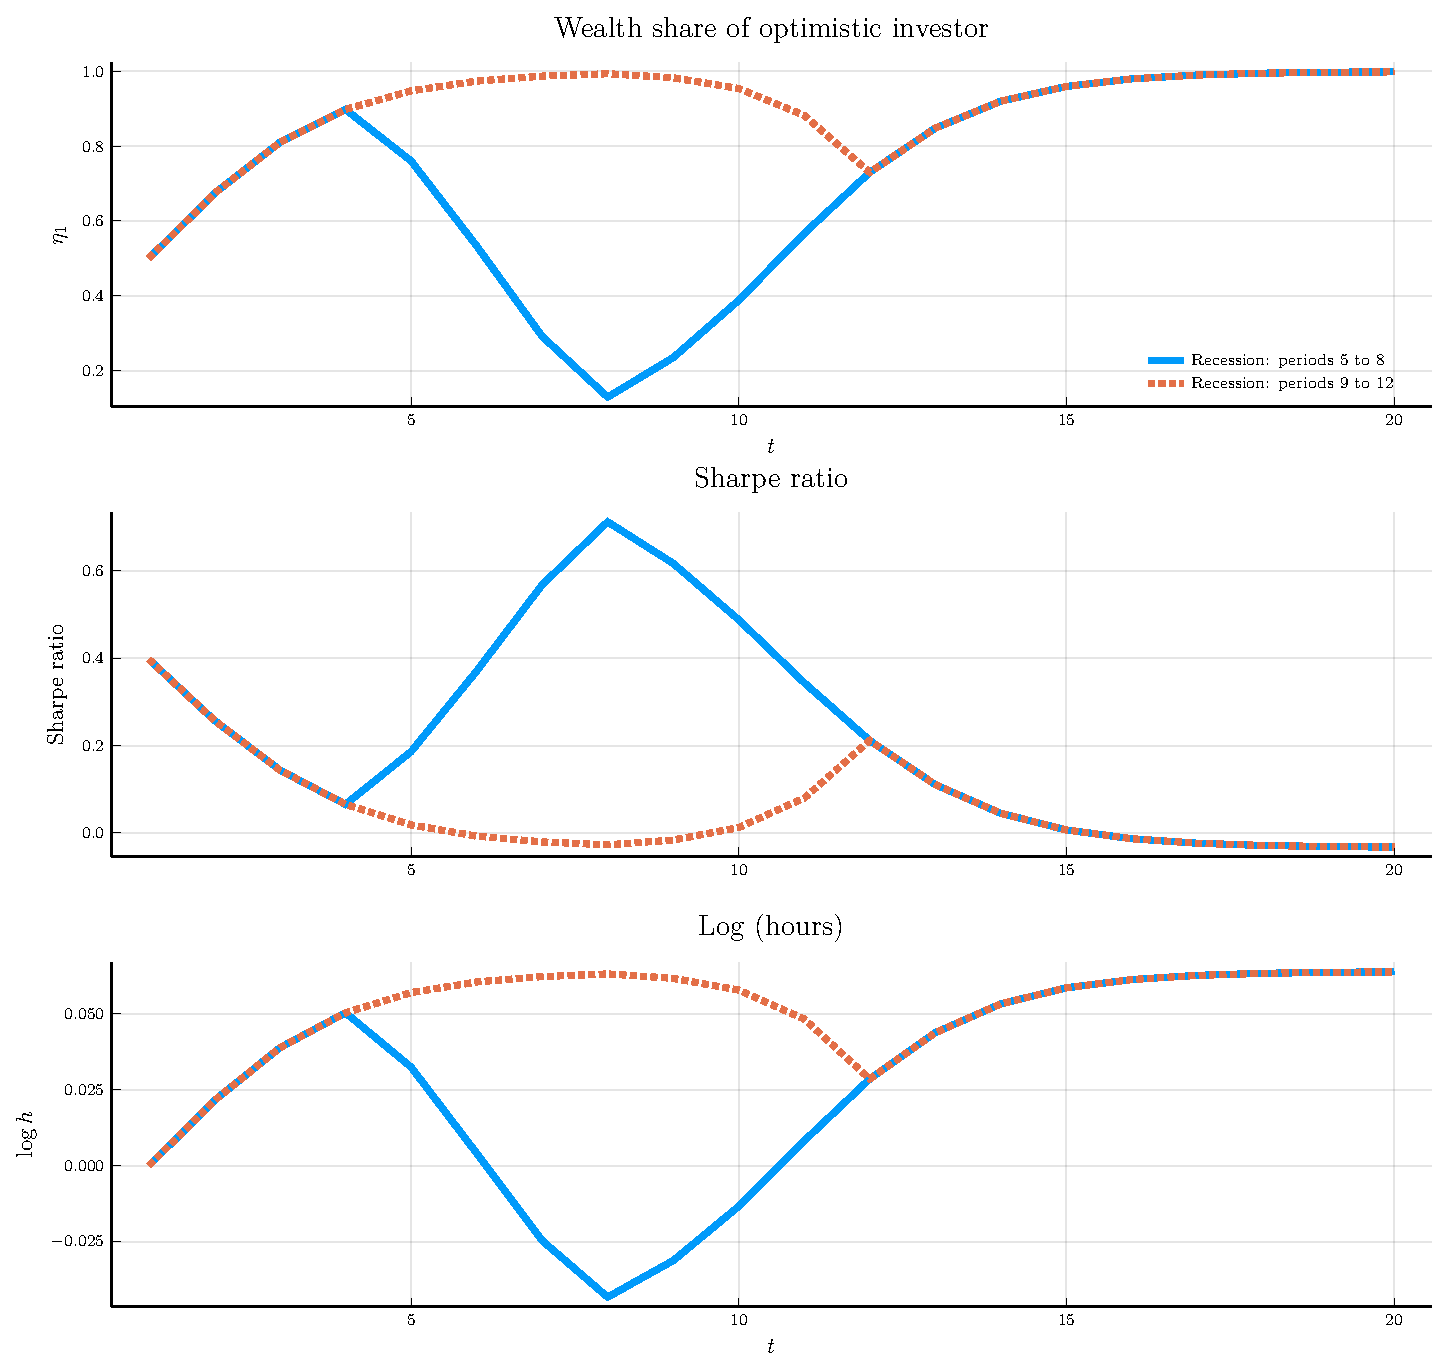
\includegraphics[width=0.75
            \textwidth]{figures/simul_het_beliefs1.pdf}
    \caption{Heterogeneous beliefs: optimistic vs pessimistic}
    \caption*{  \scriptsize 
    Note: examples of cycles (four periods of bad shocks with sixteen periods of expansions) with heterogeneous beliefs: $I=2$ investors, always optimistic and always pessimistic. The top panel shows the wealth share of the optimistic investor, the middle panel shows the Sharpe ratio (under objective beliefs), and the bottom panel shows log labor hours. \par} 
    \vspace{0.0cm}
    \label{fig: het_beliefs1}
\end{figure}

Figure~\ref{fig: het_beliefs1} illustrates this mechanism for the case of rank-preserving
beliefs. The figure shows simulations with two investors, one optimistic and one
pessimistic in all states. The top panel displays the optimist's wealth share, the middle
panel the objective Sharpe ratio, and the bottom panel log labor hours. As the economy
remains longer in the high-growth state, the optimist accumulates more wealth. 
This reduces the Sharpe ratio (i.e., the price of risk), and increases labor demand.
When the
economy eventually transitions to the low-growth state, the greater wealth share of
optimistic investors mitigates the increase in risk premia and attenuates the decline in
hours.

Figure~\ref{fig: het_beliefs2} presents the corresponding case of rank-alternating beliefs,
with one rational and one extrapolative investor. During booms, extrapolative investors
accumulate wealth, but they become pessimistic when the economy transitions to the
low-growth state. As a result, market beliefs turn sharply pessimistic during downturns,
leading to a larger increase in risk premia and a more pronounced contraction in labor
demand.
Hence, the longer the boom, the greater the bust.


\begin{figure}[t!]
    \centering
            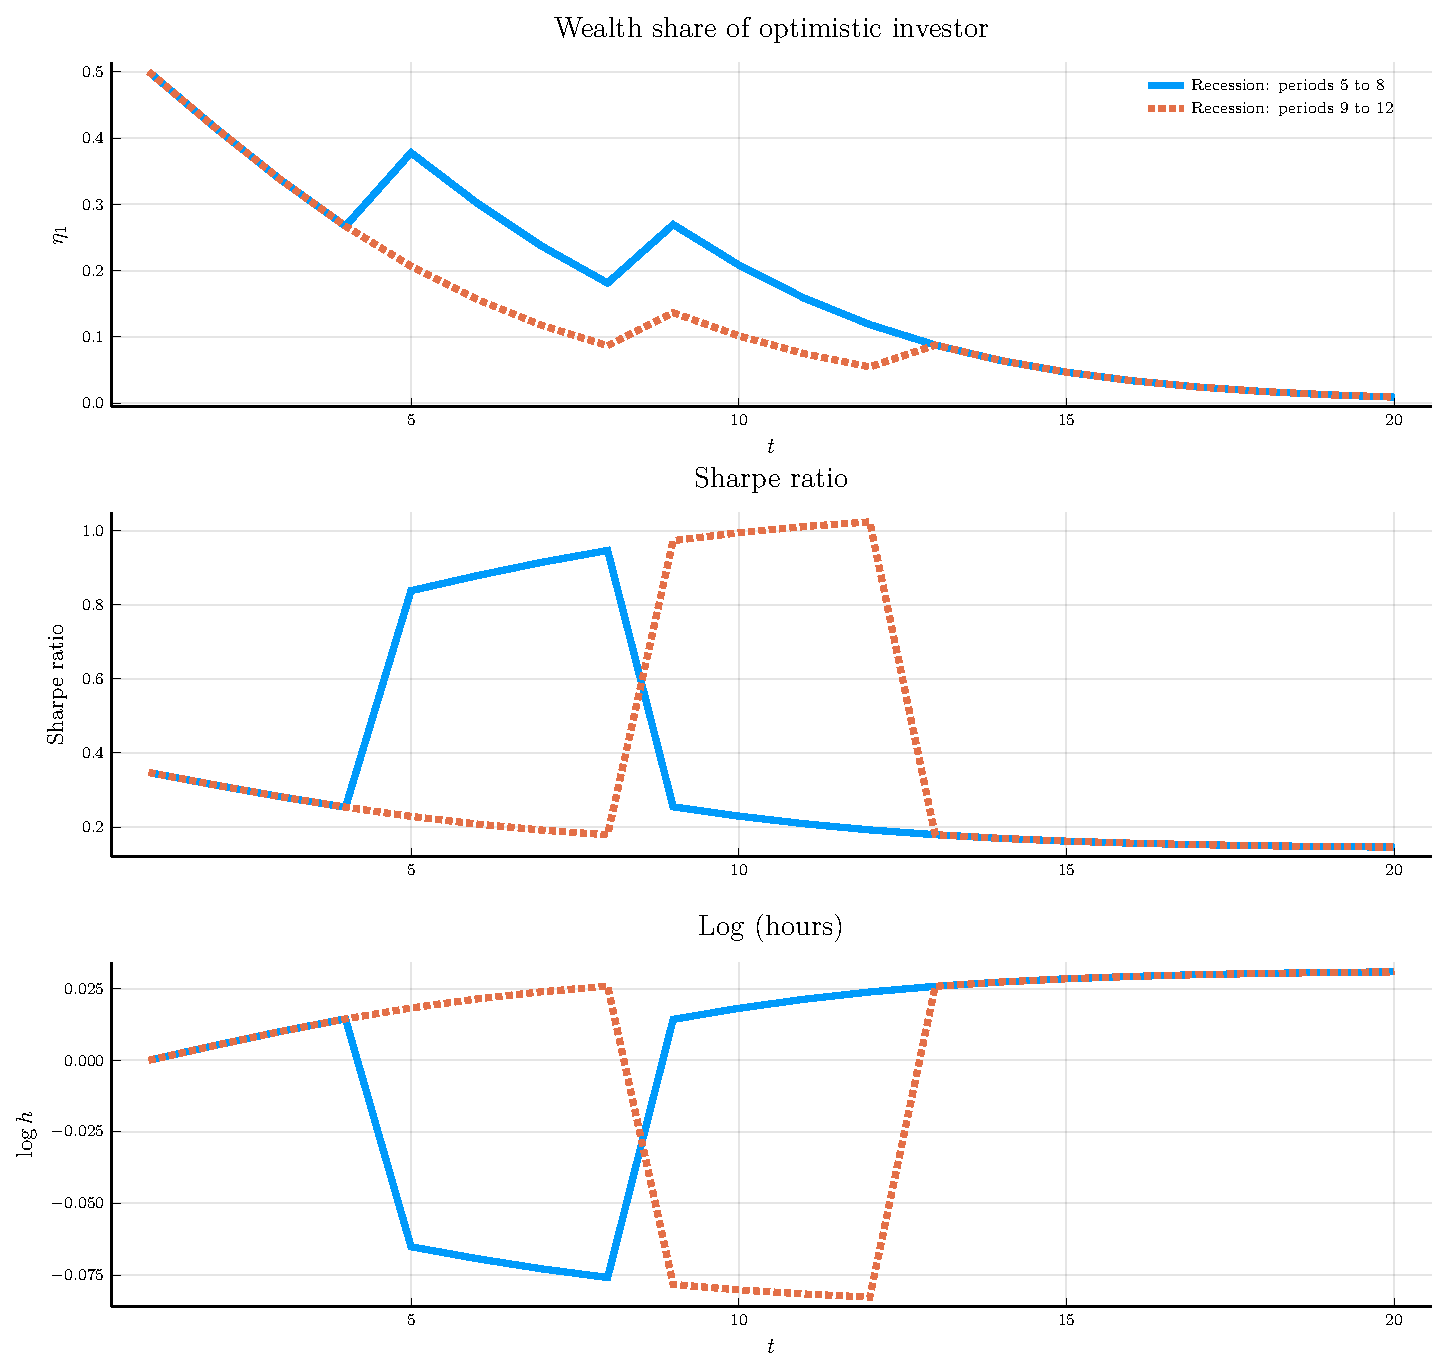
\includegraphics[width=0.75
            \textwidth]{figures/simul_het_beliefs2.pdf}
    \caption{Heterogeneous beliefs: rational vs extrapolative}
    \caption*{  \scriptsize 
    Note: examples of cycles (four periods of bad shocks with sixteen periods of expansions) with heterogeneous beliefs: $I=2$ investors, rational and extrapolative. The top panel shows the wealth share of the optimistic investor, the middle panel shows the Sharpe ratio (under objective beliefs), and the bottom panel shows log labor hours. \par} 
    \vspace{0.0cm}
    \label{fig: het_beliefs2}
\end{figure}

\q{RoleRiskAversion}{
\paragraph{The role of risk aversion.}

The results above rely on two key features of the wealth dynamics. First, the wealth
share of optimistic investors increases during booms and decreases during recessions.
Second, as implied by Proposition~\ref{prop: dynamics_beliefs}, the future wealth share of
any investor is increasing in her current wealth share:
\begin{equation}
\frac{\partial \eta_i'(X,s,s')}{\partial \eta_i}
=
\frac{p^i_{ss'}}{\overline p^m_{ss'}(X,s)}
-\eta_i\,\frac{p^i_{ss'}\bigl(p^i_{ss'}-p^I_{ss'}\bigr)}{\left(\overline p^m_{ss'}(X,s)\right)^2}
=
\frac{p^i_{ss'}}{\left(\overline p^m_{ss'}(X,s)\right)^2}
\left(\sum_{j\neq i}\eta_j p^j_{ss'}+\eta_i p^I_{ss'}\right)
\ge
0,\nonumber
\end{equation}
and it is strictly positive if, e.g., $p^j_{ss'}>0$ for all $j$.

This property contrasts with models featuring risk-neutral investors, in which optimistic
agents are driven to concentrate their wealth in the good state and are wiped
out in the bad state \citep{G10}. With risk-averse investors, by contrast,
agents choose to allocate wealth across both states of the world. As a result, optimistic
investors retain wealth in downturns, allowing the belief-driven amplification mechanism
to operate.

The strength of this mechanism depends on the degree of risk aversion. When optimistic
investors are close to risk-neutral, additional wealth accumulated during a boom is
largely tilted toward the good state, attenuating the amplification of fluctuations in
bad times. Higher risk aversion induces investors to distribute wealth more evenly across
states, increasing the influence of optimistic investors during downturns and thereby
strengthening the amplification of adverse shocks.
}

\q{FrothyMarkets}{\paragraph{Frothy markets and risk build-ups.}

An implication of Corollary~\ref{cor:het_dynamics} is that the risk premium declines
with the length of economic expansions. To the extent that risk premia are reflected
in credit spreads, the model is consistent with the discussion in
\citet{lopez2017credit} and \citet{krishnamurthy2017credit} that economic booms
are characterized by ``frothy'' market conditions driven by credit-market sentiment.

Importantly, the model delivers a joint prediction: as optimism builds during
prolonged expansions, objective risk premia decline while dividend volatility rises.
The compression in spreads reflects the greater risk-bearing capacity of optimistic
investors. At the same time, lower risk premia raise labor demand, increase the labor
share, and amplify operating leverage. Because labor is chosen in advance,
profits, and therefore dividends, become more sensitive to productivity shocks.
This combination implies an endogenous \emph{risk build-up} during booms:
fragility increases precisely when spreads are low.

As emphasized by \citet{krishnamurthy2020dissecting}, generating simultaneously
low spreads and rising risk exposure is challenging in standard macro-finance models,
such as \citet{he2013intermediary} and \citet{brunnermeier2014macroeconomic}.
In contrast, heterogeneous extrapolative beliefs naturally generate this pattern
in our framework.

Each link in this mechanism is supported by existing evidence. First, survey-based
measures of optimism are associated with lower expected returns, consistent with
compressed risk premia (e.g., \citealt{de_la_o_subjective_2021}). Second, measures of
labor demand and labor share predict lower future stock returns
(\citealt{santos2006labor, belo2023drives}), consistent with the link between labor demand
and risk premia. Third, higher labor share is associated with stronger operating leverage
and greater sensitivity of profits to shocks (\citealt{donangelo2019cross}). Taken together,
these findings support the interpretation that periods of elevated optimism are
characterized by compressed spreads and increased fragility.}
% \paragraph{Frothy markets and risk build-ups.} An implication of Corollary \ref{cor:het_dynamics} is that the risk premium declines with the length of economic expansions. 
% To the extent that risk premia drive credit spreads, the model is consistent with the discussions in \citet{lopez2017credit} and \citet{krishnamurthy2017credit} that argue that economic booms are characterized by "froth" market conditions driven by credit-market \textit{sentiments}. 
% Our framework shows that with belief extrapolation, an increase in optimism leads to a reduction in risk premia and an increase in volatility, as shown in Figure \ref{fig: risk_eq}. Under this interpretation, there is endogenous \textit{risk build-up} during booms. 
% As argued by \citet{krishnamurthy2020dissecting}, the combination of risk build-up and low spreads is challenging to generate for standard macro-finance models, such as \citet{he2013intermediary} and \citet{brunnermeier2014macroeconomic}. This observation suggests that heterogeneous extrapolative beliefs explain credit and asset-market dynamics during boom-bust cycles.

% \q{ExogenousBuildUp}{It is worth clarifying that risk-build-up requires heterogeneity only when beliefs about the state are themselves Markovian. If beliefs are history-dependent, for example, if agents become more optimistic as boom states persist but more pessimistic once the economy switches states as boom states persist, the economy can also feature risk build-up. 
%         This risk build-up would not respond to the model's internal propagation through leverage, risk-exposure, and wealth accumulation, though.}

% \paragraph{Discussion: Pareto and Belief-Neutral Welfare.} 

% \q{ParetoEfficiency}{The environment's inherent risk build-up leads to subtle normative implications. 
% It is well known that, under complete markets, the equilibrium is Pareto efficient from a subjective standpoint. 
% The First Welfare Theorem does not distinguish whether trade is driven by differences in preferences over goods or by differences in beliefs across future states--- treating both as equally valid sources of heterogeneity.} 

% \q{NeutralWelfare}{Classic Pareto efficiency is not the only sensible welfare criterion. \citet{BrunnermeierSimsekXiong2014} considers a paternalistic criterion, albeit one that does not presume superior knowledge by the planner. Instead, this belief-neutral criterion only requires the allocation to be efficient for all possible (convex combinations of) the agents' beliefs. Our environment is generically inefficient under this belief-neutral criterion: the simplest way to see this is to assume all agents believe TFP growth is iid but differ in the weights they assign states. In such a case, under all possible belief combinations, TFP growth is iid. Hence, labor fluctuations are inefficient under this criterion. This criterion can be used to justify leaning against the wind policies even though the economy is efficient in a standard sense.}


\q{RiskAversionDiscussion}{\paragraph{Discussion: belief heterogeneity vs. risk aversion.}
As discussed above, rank-alternating beliefs amplify inherent economic fluctuations.
The key distinction is that heterogeneity in beliefs can induce changes in the 
\emph{ranking} of investors' effective risk-taking across states.
In models with heterogeneous risk aversion, differences in risk tolerance can generate
portfolio dispersion and time variation in expected returns. However, the ranking of
agents in terms of risk-taking is fixed: the more risk-tolerant agent always holds
more risky assets in every state of the world. This property is analogous to the
case of rank-preserving beliefs shown in Figure~\ref{fig: het_beliefs1}.
In contrast, under rank-alternating beliefs, the identity of the relatively
risk-taking investor depends on the state. An agent who takes more risk in booms
may take less risk in busts. There is no counterpart to this mechanism in models
with heterogeneous risk aversion alone.
}

\subsection{Belief taxonomy and trading volume}\label{sec: trading_volume}
\q{TradingVolumeTheory}{

Our belief taxonomy also has sharp implications for trading dynamics. As is standard in
models with belief heterogeneity, trading volume is closely related to the degree of
disagreement among investors. We show that not only the level but also the \emph{type} of
disagreement---as classified in Definition~\ref{def: belief_taxonomy}---plays a central role
in shaping the dynamics of trading volume over the business cycle.

\subsubsection{Analytical characterization of turnover}
We adopt \emph{share turnover} as our measure of trading volume, following
\citet{lo2000trading}, defined as
\begin{equation}
    \tau_t \equiv \frac{1}{2}\sum_{i=1}^I \mu_i \big|S_{i,t}-S_{i,t-1}\big|
    = \frac{1}{2}\sum_{i=1}^I \big|\omega_{i,t}\eta_{i,t}-\omega_{i,t-1}\eta_{i,t-1}\big|,
    \nonumber
\end{equation}
where we divide by two to avoid double counting trades, and the second equality uses
$\mu_i S_{i,t}=\omega_{i,t}\eta_{i,t}$.

In the absence of belief heterogeneity, $\omega_{i,t}=1$ and $\eta_{i,t}=\eta_{i,t-1}$, so
$\tau_t=0$. With heterogeneous beliefs, turnover depends on the extent of belief dispersion.
To characterize this dependence analytically, we consider a small deviation from a
homogeneous-beliefs benchmark. Specifically, assume
\begin{equation}
    p_{ss'}^i = p_{ss'}^* + \delta_{ss'}^i \epsilon,\qquad \delta_{sH}^i+\delta_{sL}^i=0,
    \nonumber
\end{equation}
where $p_{ss'}^*$ denotes the common belief in the benchmark and $\epsilon$ controls the
degree of dispersion. For simplicity, we take the benchmark belief to be symmetric and
i.i.d., $p_{ss'}^*=\tfrac{1}{2}$. Appendix~\ref{app: proof_lemma_trading} discusses the general case.

In this neighborhood, the portfolio share and next-period wealth share of investor $i$ admit the expansions\small
\begin{equation}
    \omega_i(X,s) = 1 + \kappa_\omega\!\left[p_{sH}^i-\overline{p}^{\,m}_{sH}(X,s)\right]+\mathcal{O}(\epsilon^2),
    \qquad
    \eta_i'(X,s,s') = \eta_i + \eta_i\frac{p_{ss'}^i-\overline{p}^{\,m}_{ss'}(X,s)}{p_{ss'}^*}
    + \mathcal{O}(\epsilon^2),
    \nonumber
\end{equation}\normalsize
where $\kappa_\omega>0$ and $\overline{p}^{\,m}_{ss'}(X,s)\equiv\sum_{j=1}^I\eta_j p_{ss'}^j$
denotes market beliefs. These expressions highlight how differences in beliefs drive portfolios and wealth dynamics.

To understand the determinants of trading volume, it is useful to decompose individual
trading into two distinct components. The following lemma expresses an investor's net purchases as the sum of a rebalancing motive
and a relative belief-updating motive.

\begin{lemma}\label{lem:trading}
Investor $i$'s net purchases of shares are given by
\begin{equation}\label{eq:trading}
    \mu_i \Delta S_i(X,s,s';\epsilon)
    =
    \underbrace{\Delta \eta_i(X,s,s')}_{\text{rebalancing effect}}
    +
    \underbrace{\Delta \omega_i(X,s,s')\,\eta_i}_{\text{change-in-beliefs effect}}
    + \mathcal{O}(\epsilon^2),
\end{equation}
where\small
\begin{align}
    \Delta \eta_i(X,s,s') &\equiv \eta_i \frac{p_{ss'}^i-\overline{p}^{\,m}_{ss'}(X,s)}{p_{ss'}^*},
    \qquad
    \Delta \omega_i(X,s,s') \equiv \kappa_\omega\!\left[
        \big(p_{s'H}^i-\overline{p}^{\,m}_{s'H}(X,s)\big)
        -\big(p_{sH}^i-\overline{p}^{\,m}_{sH}(X,s)\big)
    \right].
    \nonumber
\end{align}\normalsize
\end{lemma}

Lemma~\ref{lem:trading} shows that individual trading behavior is governed by two distinct forces.
The \emph{rebalancing effect} captures trades required to maintain a constant portfolio share
following changes in relative wealth. This effect occurs because when an optimistic investor gains wealth
after a favorable shock, she must purchase additional shares to keep her portfolio composition unchanged.
The \emph{change-in-beliefs effect} reflects active portfolio reallocation driven by revisions in
relative beliefs across states: if an investor becomes more optimistic in state $s'$ than in state $s$,
she increases her exposure to the risky asset upon the transition.

Whether these two effects reinforce or offset each other depends on how beliefs evolve across states.
This interaction is the key mechanism behind the state-dependent relationship between belief dispersion
and trading volume.


\paratitle{Turnover and belief taxonomy.} As in Section~\ref{sec:environment.sec}, we can express beliefs in terms of a persistence parameter, $\rho_i$, and a bias term, $\Delta_i$:
\begin{equation}\label{eq: beliefs_persistence_bias}
    p_{HH}^i = \frac{1+\rho_i}{2} + \Delta_i, \qquad \qquad p_{LH}^i = \frac{1-\rho_i}{2} + \Delta_i,\nonumber
\end{equation}
which implies that the conditional expectation of productivity growth is given by:
\begin{equation}\label{eq: conditional_expectation}
    \mathbb{E}_{i,t}[x_{t+1}] = \overline{x}_i + \rho_i (x_t - \overline{x}_i),
\end{equation}
where $\overline{x}_i$ is the subjective unconditional mean of $x_t$.

Consider first the case of rank-preserving beliefs, $\rho_i = \rho$, where investors differ on the level of optimism, $\Delta_i$. 
% In this case, beliefs are constant, $p_{HH'}^i = p_{LL'}^i = \frac{1+\rho}{2}$, and turnover is given by:
In this case, the change-in-beliefs effect vanishes and turnover is driven
solely by the rebalancing effect:
\begin{equation}
    \tau(X,s,s';\epsilon)
    =
    \sum_{i=1}^I \eta_i
    \big|p_{ss'}^i-\overline{p}^{\,m}_{ss'}(X,s)\big|
    +\mathcal{O}(\epsilon^2).
    \nonumber
\end{equation}
In this case, turnover is proportional to the average absolute deviation of beliefs, a natural
measure of belief dispersion, so trading volume increases with disagreement.

Consider next the case of rank-alternating beliefs, $\Delta_i = \Delta$, where investors differ on the persistence parameter, $\rho_i$. 
In this case, the change-in-beliefs effect emerges when the economy switches states, $s\neq s'$, and it may either
amplify or dampen the rebalancing effect. 
For instance, suppose the
economy switches from $H$ to $L$. Investors who were relatively
optimistic in the boom lose wealth on impact and, at the same time, become relatively pessimistic in
the downturn. Both forces push toward selling, so turnover rises sharply. By contrast, when the
economy switches from $L$ to $H$, the same investors become relatively optimistic and wish to raise
their risky share, while rebalancing incentives work in the opposite direction because their wealth share decreases. Turnover is therefore more sensitive to disagreement in recessions than in expansions.

% To formalize this asymmetry, consider a rank-alternating specification in which investors agree on the
% unconditional mean of productivity growth, $\overline{x}$, but disagree about persistence, $\theta_i$:
% \begin{equation}\label{eq: persistence}
%     \mathbb{E}_{i,t}[x_{t+1}] - \overline{x} = \theta_i\,(x_t-\overline{x}),
% \end{equation}
% where $\theta_i$ is a function of $p_{ss'}^i$. 
The next proposition formalizes this intuition and delivers the central result of this
section: trading volume is increasing in belief dispersion, and this relationship is asymmetric over the
business cycle under rank-alternating beliefs.

\begin{proposition}\label{prop:turnover}
Suppose investors' beliefs are rank-alternating, that is, they are given by \eqref{eq: beliefs_persistence_bias} with $\Delta_i = \Delta$. Turnover as the economy switches from $s$ to $s'$ is given by
\begin{equation}
    \tau(X,s,s';\epsilon)
    =
    \frac{\zeta(s,s')}{2}\sum_{i=1}^I \eta_i \big|\rho_i-\rho(X)\big|
    +\mathcal{O}(\epsilon^2),
    \nonumber
\end{equation}
where $\rho(X) \equiv \sum_{i=1}^I \eta_i \rho_i$, and
\begin{equation*}
    \zeta(s,s') \equiv
    \left\{
    \begin{array}{ll}
        \kappa_\omega+1, & \text{if } s=H \text{ and } s'=L,\\
        \big|\kappa_\omega-1\big|, & \text{if } s=L \text{ and } s'=H,\\
        1, & \text{if } s=s'.
    \end{array}
    \right.
\end{equation*}
\end{proposition}

The key message from Proposition~\ref{prop:turnover} is that turnover increases with belief dispersion and,
furthermore, that this sensitivity is stronger in downturns. The assumption of rank-alternating beliefs is essential for generating this asymmetry. With rank-preserving beliefs---investors are relatively
optimistic or pessimistic by the same amount in both states---the change-in-beliefs effect is absent, and turnover is driven primarily by rebalancing. Hence, disagreement does not generate a disproportionately strong response of trading volume in bad times. Thus, rank-alternating beliefs are key to inducing state-dependent dynamics of stock market turnover.
}


\subsubsection{Empirical evidence}

\begin{figure}[t!]
    \caption{Disagreement Index and Stock Market Turnover}
    \centering
    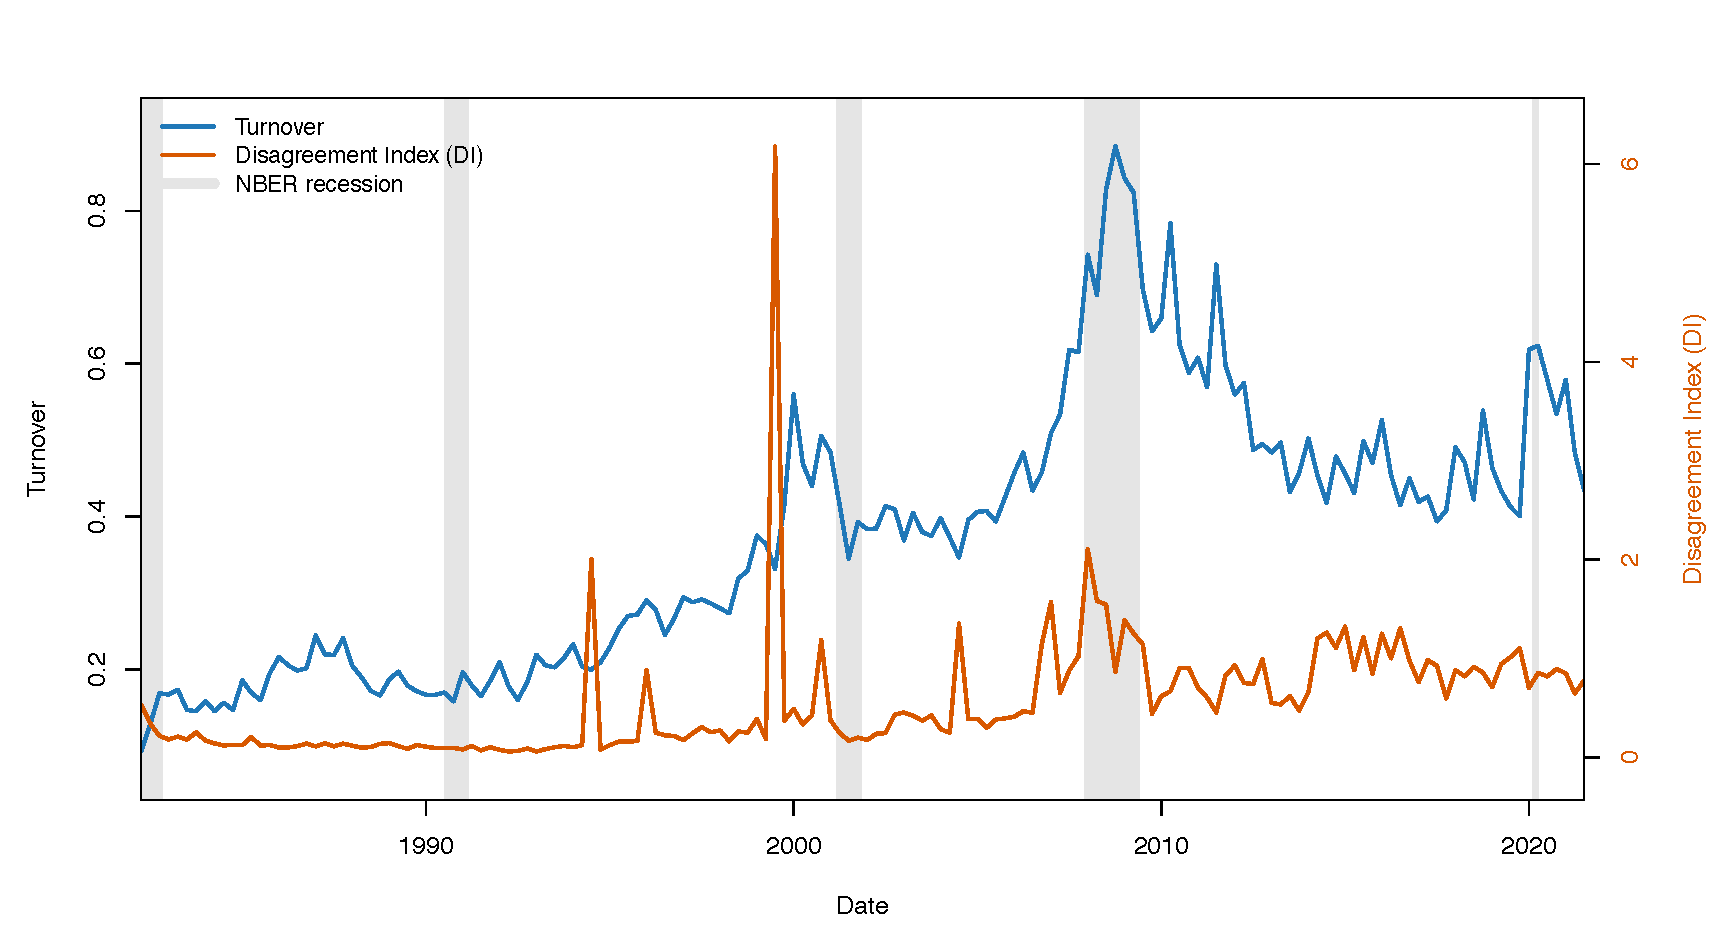
\includegraphics[width=0.9\textwidth]{figures/turnover_vs_disagreement_index.pdf}
    \label{fig: DI_turnover_time_series}
\end{figure}

\q{EmpiricalEvidenceI}{We now test the model's prediction that trading volume increases with belief
dispersion and that this sensitivity is stronger during downturns.

\paragraph{Measuring disagreement and turnover.}

The model links trading dynamics to disagreement about aggregate shocks.
To construct an empirical analogue, we combine analyst forecasts from I/B/E/S
with stock market turnover from CRSP.

Let $\mathbb{E}_{j,t}[\Delta e_{i,t+1}]$ denote analyst $j$'s forecast of
firm $i$'s earnings growth at time $t$, and let $\Delta e_t$
denote realized aggregate earnings growth.
To isolate the analyst-specific component reflecting beliefs about aggregate dynamics,
we estimate
\begin{equation}
    \mathbb{E}_{j,t}[\Delta e_{i,t+1}]
    =
    \alpha_{i,t}
    +
    \beta_{0,j}
    +
    \beta_{1,j} \Delta e_t
    +
    u_{j,i,t},
\end{equation}
where $\alpha_{i,t}$ is a firm--time fixed effect,
$\beta_{0,j}$ is an analyst-specific intercept,
$\beta_{1,j}$ captures the analyst's sensitivity to aggregate earnings growth,
and $u_{j,i,t}$ is an error term.

The firm--time fixed effect absorbs firm-level information common to all analysts.
The remaining analyst-specific terms therefore capture systematic differences in beliefs
about aggregate earnings dynamics.
We interpret the implied aggregate expectation of analyst $j$ as
\[
\mathbb{E}_{j,t}[\Delta e_{t+1}]
=
\beta_{0,j} + \beta_{1,j} \Delta e_t,
\]
which mirrors the model's specification of expected productivity growth
in Equation~\eqref{eq: conditional_expectation}.

We then construct a time-varying \emph{disagreement index} as the cross-sectional
dispersion of these implied aggregate expectations:
\begin{equation}
    DI_t
    =
    \overline{\sigma}_t\!\left[\beta_{0,j} + \beta_{1,j} \Delta e_t \right],
\end{equation}
where $\overline{\sigma}_t[\cdot]$ denotes the cross-sectional standard deviation at time $t$. 

While analyst-specific coefficients are constant over time, time changes in disagreement occur through $\Delta e_t$. This reflects the model's mechanism that dispersion in persistence beliefs interacts
with the current state of the economy.

To measure trading activity, we follow \citet{lo2000trading} and compute
value-weighted stock market turnover from CRSP.\footnote{
Details on construction are provided in Appendix~\ref{app:data_turnover}.}

Figure~\ref{fig: DI_turnover_time_series}
plots the time series of the disagreement index and turnover.
Shaded areas correspond to NBER recessions.
Disagreement rises sharply in downturns,
periods in which turnover is also elevated.}


\begin{table}[!t]\centering
    \caption{Turnover Regressions with Standardized Disagreement}
    \label{tab:turnover_di_5specs_standardized}
    
    \resizebox{\textwidth}{!}{%
    \begin{tabular}{lccccc}
    \hline\hline
     & Baseline & Rec $\times$ DI & Rec $\times$ DI 
     & Early Rec. & Early Rec. \\
     & (1) & (2) & (3) & (4) & (5) \\
    \hline
    Disagreement (z-score) 
        & 0.075 & 0.054 & 0.054 & 0.069 & 0.069 \\
        & (0.047) & (0.039) & (0.039) & (0.047) & (0.047) \\
    
    Recession 
        &  & 0.051 &  &  &  \\
        &  & (0.048) &  &  &  \\
    
    Disagreement $\times$ Recession 
        &  & 0.176*** & 0.188*** &  &  \\
        &  & (0.058) & (0.061) &  &  \\
    
    Early Rec. (first 2 qtrs) 
        &  &  &  & 0.014 &  \\
        &  &  &  & (0.035) &  \\
    
    Disagreement $\times$ Early Rec. 
        &  &  &  & 0.095* & 0.098* \\
        &  &  &  & (0.051) & (0.051) \\
    
    \hline
    Marginal effect of DI in recession 
        &  & 0.230 & 0.242 & 0.164 & 0.167 \\
    
    Constant 
        & 0.311*** & 0.301*** & 0.305*** & 0.309*** & 0.309*** \\
        & (0.023) & (0.022) & (0.020) & (0.023) & (0.022) \\
    
    \hline
    Observations & 158 & 158 & 158 & 158 & 158 \\
    $R^2$ & 0.212 & 0.352 & 0.344 & 0.235 & 0.235 \\
    \hline\hline
    \end{tabular}%
    }
    
    \vspace{0.2em}
    {\begin{flushleft}
        \footnotesize
        Sample period: 1982Q2--2021Q3. Disagreement is standardized within sample.
        Newey--West (lag 4) standard errors in parentheses.
        * $p<0.10$, ** $p<0.05$, *** $p<0.01$.
        \end{flushleft}}
    
    
    \end{table}


\q{EmpiricalEvidenceII}{\paragraph{Regression evidence.}

We formally assess the relationship using time-series regressions of turnover on
the standardized disagreement index $DI_t$.
Table~\ref{tab:turnover_di_5specs_standardized}
reports Newey--West standard errors with four lags: Column (1) shows a positive but statistically insignificant association between
turnover and disagreement.
Column (2) adds an NBER recession indicator and its interaction with disagreement.
The interaction term is positive and highly significant,
indicating that turnover becomes substantially more sensitive to disagreement in recessions.
The implied marginal effect of disagreement during recessions
is economically meaningful: a one-standard-deviation increase in $DI_t$
is associated with an increase in turnover of approximately
$0.23$ (the sum of the main and interaction coefficients),
a sizeable fraction of its sample mean $(0.31)$.
This is exactly what  Proposition~\ref{prop:turnover} predicts: the turnover--disagreement relationship strengthens in recessions.

Column (3) shows that the interaction effect remains substantial when the recession dummy
is excluded, indicating that the result is driven by differences in slopes rather than by shifts in the intercept.

The model emphasizes the role of state transitions in generating this asymmetry.
To proxy for transition periods,
Columns (4) and (5) focus on the first two quarters of NBER recessions.
Although the number of such observations is smaller,
the interaction between disagreement and the transition indicator
remains positive and statistically significant.
This evidence is consistent with the model's prediction that
turnover responds most strongly to disagreement at the onset of downturns.

The results are robust to controlling for aggregate market volatility (VIX)
and market returns; these specifications are reported in Appendix~\ref{app:data_turnover}. Overall, the evidence supports the model's central implication:
while trading volume increases with belief dispersion,
this sensitivity is substantially stronger in recessions,
particularly around state transitions.
}
        
    


% \subsection{Belief heterogeneity and stock market turnover.}  

% Here we present an econometric analysis to measure belief heterogeneity and relate this heterogeneity with stock-market turnover.
  
% \paragraph{A process for realized and expected earnings.}

% % consolidate notation with data explaination above.
% Let $i \in \mathcal{I}$ denote a firm-analyst observation in the I/B/E/S data---we index firm-level outcomes also by $i$. We denote (realized) earnings for $i$ at period $t$ by $e_{i,t}$  and its first-difference by $\Delta e_{i,t} = e_{i,t} - e_{i,t-1}$.\footnote{As $e_{i,t}$ can potentially be negative, we work with first differences instead of proportional differences, $\frac{\Delta e_{i,t}}{e_{i,t}}$, or log-differences, $\Delta \log (e_{i,t})$. By focusing on first differences, we do not have to drop firms which experience negative earnings, which is a significant fraction of our sample.}
% % \todo{maybe we should say why we did not standarize. Would be ideal to introduce notation above once.} In turn, we denote aggregate earnings by $e_t$ and the first-difference of aggregate earnings by $\Delta e_t$. We specify a process for the realized earnings of $i$ in terms of an exposure to the aggregate earnings:
% \begin{equation}\label{eq: realized_earnings}
%     \Delta e_{i,t} = \beta_i \Delta e_t + u_{i,t},
% \end{equation}
% where $u_{i,t} = \rho_i u_{i,t-1} + \epsilon_{i,t}$ and $\epsilon_{i,t} \sim \mathcal{N}(0, \sigma_{\epsilon}^2)$.  The error term $\epsilon_{i,t}$ is i.i.d. and independent of $\Delta e_t$.\footnote{For exposition, we assume that $\Delta e_{i,t}$ and $\Delta e_t$ have already been de-meaned, so we can omit the intercept, and that $\Delta e_{i,t}$ and $\Delta e_t$ have been normalized to have unit variance.}
% Idiosyncratic shocks are captured by $u_{i,t}$. In turn, $\rho_i$ controls the persistence of idiosyncratic shocks. Hence, we assume that all firms are heterogeneous regarding their exposure to the aggregate earnings shock and the persistence of their idiosyncratic shocks. 

% To exploit the cross-section of the data, we focus on disagreement regarding the persistence of the shocks to aggregate earnings. For that, we assume that analysts agree that their stocks' earnings are exposed to the aggregate factor following \eqref{eq: realized_earnings}, but disagree on the process for aggregated earnings. In particular, we assume that analyst $i$ believes (in a  dogmatic fashion) that  $\Delta e_t$ follows:
% \begin{equation}
%     \Delta e_{t} = \theta_i \Delta e_{t-1} + \nu_{i,t}, 
% \end{equation}
% where $\nu_{i,t}$ is an i.i.d. process given by $\nu_{i,t} \sim \mathcal{N}(0, \sigma_\nu^2) $. Analysts agree on the unconditional mean for $\Delta e_t$, which we normalized to zero and  $\Delta e_{t}$ is perfectly observed. Thus, the expected change in aggregate earnings of analyst $i$ is given by
% \begin{equation}
%     \mathbb{E}_{i,t}[\Delta e_{t+1}] = \theta_i \Delta e_{t},
% \end{equation}
% where $\mathbb{E}_{i,t}[\cdot]$ denotes the conditional expectation at $t$ of $i$. Hence, differences in beliefs are exclusively captured by differences regarding $\theta_i$, the mean-reversion of aggregate earnings. For example, the formulation can capture belief extrapolation: a high value for $\theta_i$ implies that $i$ is more optimistic about aggregate earnings after a positive shock and more pessimistic after a negative shock, that an agent with a lower $\theta_j$.   
% % cite evidence? or say, has ben argued that matters. maybe bring up to justify assumption?

% Expectations of changes in \textit{individual} earnings depend on 
% %the degree of persistence of shocks to \textit{aggregate} earnings 
% $\theta_i$:
% \begin{equation}\label{eq: subjective_expectations_individual}
%     \mathbb{E}_{i,t}[\Delta e_{i,t+1} ] = \beta_i \theta_i \Delta e_t + \rho_i u_{i,t}.
% \end{equation}
% Equation \eqref{eq: subjective_expectations_individual} shows that we can infer properties of the unobserved process for subjective beliefs on \textit{aggregate} earnings using the information on observed subjective beliefs about \textit{individual} earnings. 

% We estimate $\{\beta_i, \rho_i, \theta_i\}_{i=1}^I$ using a multi-level Bayesian model. We describe the estimation procedure in detail in Appendix \ref{app:estimation_heterogeneity}.\footnote{The procedure is analogous to a ridge regression, where the estimates are regularized using a L2 penalty (see e.g. \citealp{hastie2009elements}).}  

% \paragraph{A summary series of belief disagreement.}

% To relate belief disagreement with stock turnover, we first construct a measure of the former. Recall that the expectation of analyst of aggregate earnings growth is given by $\mathbb{E}_i[\Delta e_{t+1}] = \theta_i \Delta e_t$. 
% Hence, we use the following \textit{disagreement index} $DI_t$,:
% \begin{equation}
%     DI_t = \underbrace{\overline{\sigma}[\theta_i] \times | \Delta e_t | }_{\overline{\sigma}[\mathbb{E}_i[\Delta e_{t+1}] ] }.
% \end{equation}
% % \begin{figure}[t!]
% %     \caption{Kernel estimate of cross-sectional distribution of the different parameters}
% %     \begin{center}
% %             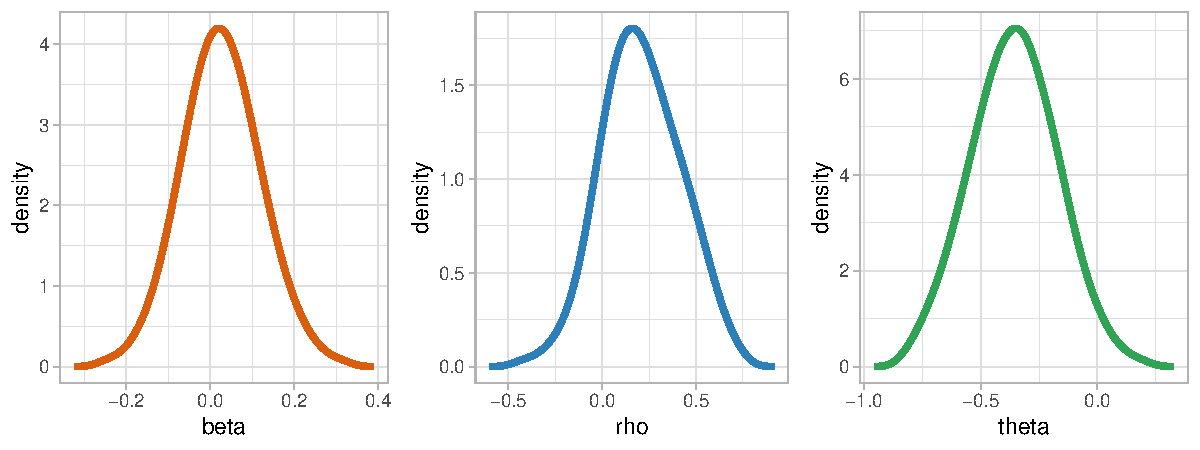
\includegraphics[width=1.0\textwidth]{figures/kernel_densities.pdf}
% %     \end{center}
% %     \caption*{  \scriptsize Note: Posterior mean of the kernel density for the cross-section of $\theta_i$ (left panel), $\rho_i$ (middle panel), and $\theta_i$ (right panel).\par} 
% %     \vspace{0.0cm}
% %     \label{fig: kernel_estimates}
% % \end{figure}
% The disagreement index (DI) has two components: First, the cross-sectional dispersion in $\theta_i$. 
% Second, the absolute value of current aggregate earnings growth, $|\Delta e_t|$. If all analysts agree on the persistence of aggregate earnings growth, such that $\overline{\sigma}[\theta_i] = 0$, then the DI would equal to zero. In turn,given that $\Delta e_t$ has been already de-meaned, $|\Delta e_t|$ captures the distance of aggregate earnings growth to the mean. 
% If aggregate earnings growth is at its average value, $|\Delta e_t| = 0$, there is no disagreement. Thus, the DI depends on the interaction deviations from mean of aggregate earnings and the underlying disagreement about the speed of reversal.  

% The left panel of Figure \ref{fig: DI_turnover_time_series} shows the time series of DI. Disagreement is low during expansions, but spikes in recessions, the periods where earnings growth deviates most from mean. 

% \paragraph{Turnover.} Theories of belief disagreement theories relate to stock-market turnover. We relate the value-weighted stock-market turnover with the DI.
% % \footnote{For a discussion of turnover as a measure of trading volume and its connection with standard portfolio theory, see \citet{lo2010stock}.} 
% \footnote{We measure the stock turnover - shares traded divided by shares outstanding---for individual securities on the New York and American Stock Exchanges from January 1977  to December 2021. We measure turnover at the quarterly frequency and compute an aggregate turnover measure using a value-weighted average (similar results are obtained by using an equal-weight measure).}
% The right panel of Figure \ref{fig: DI_turnover_time_series} shows the time series of turnover. Turnover increased significantly over time, but more importantly for our purposes, shows an important countercyclical behavior.
% % potentially reflecting an increase in market participation, 
% %, as shown by the difference between the turnover and its HP-filtered trend.

% \begin{figure}[t!]
%     \caption{Time series of the disagreement index and stock market turnover}
%     \begin{center}
%             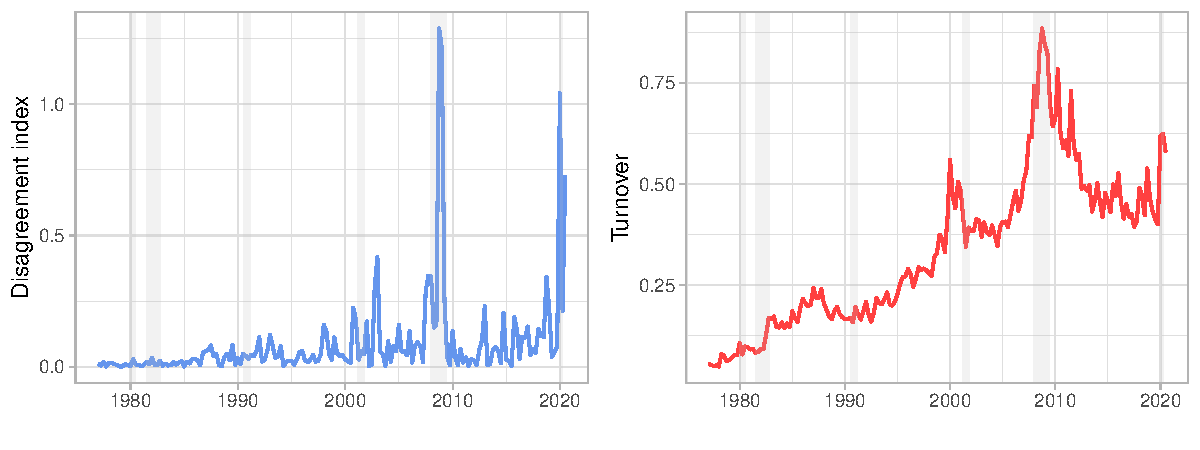
\includegraphics[width=1.0\textwidth]{figures/DI_turnover_time_series.pdf}
%     \end{center}
%     \caption*{  \scriptsize Note: Left panel shows the time series of the disagreement index and the right panel shows the time-series of stock market turnover. The smooth line in the right panel is the HP-filter trend of turnover. The vertical bars represent NBER recessions.\par} 
%     \vspace{0.0cm}
%     \label{fig: DI_turnover_time_series}
% \end{figure}

% Next, we compare the DI with turnover. 
% Table \ref{tab:reg_turnover_DI} shows the result of a time-series regression of turnover against the DI. As shown in Figure \ref{fig: DI_turnover_time_series}, the disagreement DI features outliers particularly during recessions. We thus exclude observations where the DI is below the $2.5\%$ percentile or above the $97.5\%$ percentile. 
% Column (1) shows a strong statistically significant correlation between DI and turnover.
% % SB: ---we compute Newey-West standard-errors with four lags. To bottom of table!
% If the disagreement index increases from the $25\%$ percentile value to its $75\%$ percentile value, turnover increases
% % by $8.0$ percentage points, an increase of 
% by almost $30\%$. 
% Column (2) shows that turnover responds particularly strongly to the DI during downturns. 
% We add an interaction of the DI with a dummy for NBER recessions and find that the coefficient is positive and statistically significant; its magnitude is economically large, the response of turnover to the DI is $70\%$ larger in recessions. 
% Column (3) tests for a nonlinear relationship: we introduce a quadratic term, again excluding outliers. The quadratic term is non significant. %, consistent with a linear relationship---see also Figure \ref{fig: DI_turnover_scatter}, which shows the scatterplot of turnover and the disagreement index for this sample.
% However, Column (4) performs the same non-linear regression but including outliers. In this case, the quadratic term becomes statistically significant, again indicating that the outliers also capture increased disagreement during downturns. 
% % The magnitude of the linear terms in the regressions is similar in all cases. 

% We conclude this analysis a remark: 
% \begin{remark}
% The DI is strongly correlated with turnover, but more so in crises. 
% \end{remark}
% In the theory section, connect this evidence with the predictions of different belief models.

% \begin{table}[t!]
%     	\centering
%     	\caption{Regression of turnover on disagreement index}
%  	\begin{tabular}{lcccc}
%    \tabularnewline \midrule \midrule
%    Dependent Variable: & \multicolumn{4}{c}{$turnover$}\\
%    Model:         & (1)            & (2)            & (3) & (4)\\  
%    \midrule
%    \emph{Variables}\\
%    (Intercept)    & 0.258$^{***}$ & 0.262$^{***}$ & 0.242$^{***}$ & 0.255$^{***}$\\   
%                   & (0.034)      & (0.042)       & (0.044)       & (0.037)\\   
%    $DI$             & 1.239$^{***}$  & 1.066$^{**}$  & 1.798$^{**}$  & 1.260$^{***}$\\   
%                   & (0.228)       & (0.628)       & (0.628)       & (0.290)\\   
%    $DI \times $ recession   &      & 0.742$^{**}$  &          & \\   
%                   &                & (0.253)        &         & \\       
%    $DI^2$            &             &          & -2.068         & -0.688$^{**}$\\   
%                   &                &         & (1.692)        & (0.209)\\   
   
%    \midrule
%    \emph{Fit statistics}\\
%    Observations   & 165            & 165            & 165            & 175\\  
%    R$^2$          & 0.24084        & 0.26430        & 0.24786        & 0.30386\\  
%    Adjusted R$^2$ & 0.23618        & 0.25522        & 0.23857        & 0.29576\\  
%    \midrule \midrule
%    \multicolumn{4}{l}{\emph{Newey-West standard-errors in parentheses (4 lags)}}\\
%    \multicolumn{4}{l}{\emph{Signif. Codes: ***: 0.01, **: 0.05, *: 0.1}}\\
% \end{tabular}
% \caption*{  \scriptsize Note: Columns (1) and (2) .\par} 
%     \label{tab:reg_turnover_DI}
% \end{table}





%%%%%%%%%%%%%%%%%%%%%%%%%%%%%%%%%%%%%%%%%%%%%%%%%%%%%%%%%%%%%%%%%%%%%%%%%%%%%%%%%%%%%%%%%%%%%%%



% \begin{figure}[t!]
%     \caption{Scatterplot of the disagreement index and stock market turnover}
%     \begin{center}
%             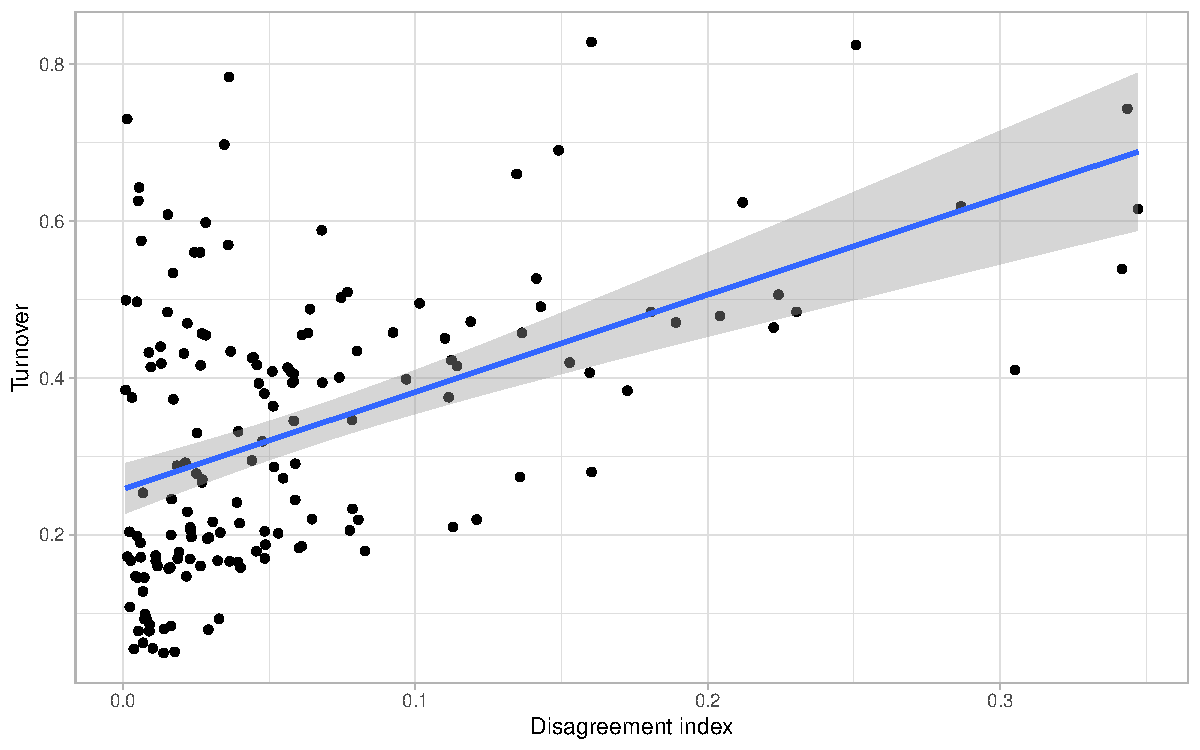
\includegraphics[width=0.8\textwidth]{figures/DI_turnover_scatter.pdf}
%     \end{center}
% %    \caption*{  \scriptsize Note: .\par} 
%     \vspace{0.0cm}
%     \label{fig: DI_turnover_scatter}
%     \caption*{  \scriptsize Note: Scatterplot of disagreement index and turnover for a sample without outliers.\par} 
% \end{figure}



% \paragraph{Connecting with the Turnover Evidence.}
% It is convenient to express heterogeneity in beliefs, $p_{ss}^i$, in terms of heterogeneity in the perceived \textit{persistence} of fundamentals. Assuming investors agree on the unconditional mean of $x_t$, $\overline{x}$, we can write $\mathbb{E}_{i,t}[x_{t+1}] - \overline{x} = \theta_i (x_t - \overline{x})$, where $\theta_i$ is a function of $p_{ss'}^i$.
% % We can recast beliefs about $p_{ss}^i$ into beliefs about mean reversion rates in earning growth, $\theta^i$---as estimated in Section \ref{sec:quantitative}. 
% The following corollary shows heterogeneous beliefs lead to larger turnover rates as the economy switches from booms to recessions.
% \begin{corollary}\label{cor: turnover} Suppose investors agree on the unconditional mean of $x_t$, i.e. $p_{LH}^i / p_{HL}^i = \overline{p}_H / \overline{p}_L$ and that the following condition is satisfied: $p_{ss'}^* = \overline{p}_H = \frac{1}{2}$. Turnover as the economy switches from $s$ to $s'$ is given by
% \begin{equation}
%     \tau(X,H,L;\epsilon) = \frac{\zeta(s,s')}{2}\sum_{i=1}^I \eta_i |\theta_i - \theta(X)| + \mathcal{O}(\epsilon^2),
% \end{equation}
% where
% \begin{equation*}
%     \zeta(s,s') \equiv \left\{ 
%     \begin{matrix}
%     \kappa_\omega + 1, \qquad & \text{if } $s = H$ \text{ and } $s' = L$\\
%     |\kappa_\omega - 1|, \qquad & \text{if } $s = L$ \text{ and } $s'  = H$\\
%     1, \qquad & \text{if } $s = s'$
%     \end{matrix}
%     \right. 
% \end{equation*}
% \end{corollary}
% % The assumption $p_{ss'}^* = \overline{p}_H = \frac{1}{2}$ is made only to simplify the presentation. The general case is considered in the appendix.
%  The key message from Corollary \ref{cor: turnover} is that turnover increases in belief dispersion and, furthermore, that the effect is more pronounced during busts. 
% Both predictions are in line with the evidence discussed in Section \ref{app_disagreement_evidence}. The assumption of rank-alternating beliefs is important to obtain this asymmetric effect. 
% If investors have rank-preserving beliefs, where they are equally optimistic or pessimistic in both states, so $\tilde{\delta}_{s'H}^i = \tilde{\delta}_{sH}^i $ even for $s'\neq s$, then the change-in-beliefs effect will be equal to zero and we would not obtain a stronger response of turnover to disagreement during bad times. Therefore, rank-alternating beliefs are key to capturing the dynamics of stock market turnover. 

% Our taxonomy also has implications for trading dynamics.
% As is typical in models of belief heterogeneity, trading volume increases with the level of belief disagreement.
% More importantly, Appendix~\ref{app:volume} shows that the relationship between trading volume and belief disagreement is amplified during economic downturns under \textit{rank-alternating} beliefs, not under \textit{rank-preserving} beliefs. 
% The intuition is as follows: optimistic investors lose wealth and rebalance their portfolios by selling shares when the economy enters a recession. 
% If their beliefs are rank-alternating, they also become pessimistic, which induces additional selling, further increasing trading volume.
% % Intuitively, optimistic investors lose wealth as the economy switches to the bad state, so they rebalance their portfolios by selling shares. 
% % If they have rank-alternating beliefs, they also become pessimistic, leading to an additional selling of shares, further increasing trading volume.
% Appendix~\ref{app:belief_heterogeneity_estimation} provides empirical support for this prediction. 
% We find that not only does stock market turnover rise with belief disagreement, but this relationship also strengthens during recessions, consistent with the predictions under rank-alternating beliefs.
